\section{Method of alignment for the RICH optical system}
\label{sec:MirrorAlignmentMethod}

Photons are ``reconstructed''  from hits on the photon detector plane by
reflecting  them off the \rich mirrors, based on the \rich geometry information
available to the \lhcb reconstruction software. For definiteness, the photons
are assumed to originate from the midpoint of a track as it traverses the \rich
radiator. This assumption allows a Cherenkov angle to be calculated.

A misalignment of the \lhcb \rich optical system manifests itself as a
displacement of the observable Cherenkov ring against the expected one
\cite{Papanestis:2008zz, Baldini:2006ed}. In other words, a discrepancy occurs
between the actual centre of the Cherenkov ring and its expected position
calculated from the reconstructed tracks momentum and using pion mass
hypothesis.  This is explained in \fig{fig:RICH_MisalignmentDiagrams} and its
caption (partly inspired by the respective figure from~\cite{Gorisek:1999td}).
\begin{figure}[hbt]
  \vspace{-0.5\baselineskip}
  \centering{
    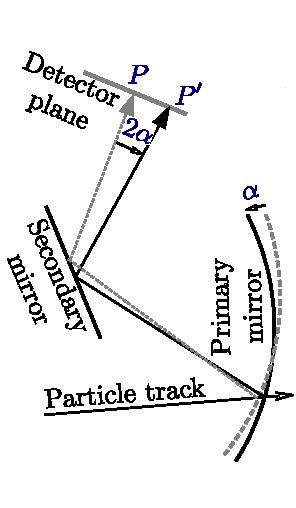
\includegraphics[width=0.27\textwidth]{figs/Method/TiltedMirror}
    \hspace{0.07\textwidth}
    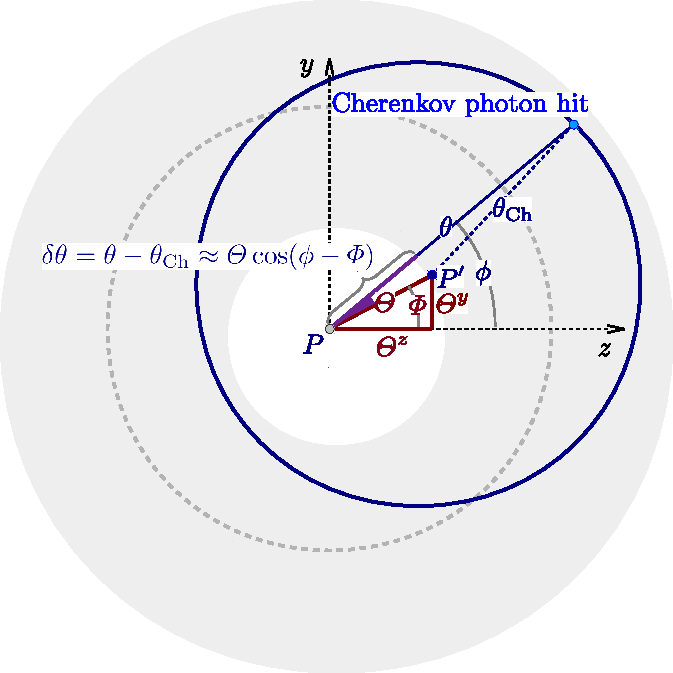
\includegraphics[width=0.61\textwidth]{figs/Method/ShiftedRing_andStripe}
  }
  \hspace{0.35\textwidth}(a)\hspace{0.52\textwidth}(b)\hspace{0.13\textwidth}
  \vspace{-0.5\baselineskip}
  \caption{
    (a) Schematic drawing of how rotational misalignment of a \rich mirror
    (primary mirror in this example) causes shift of the actual centre $P'$ of
    the Cherenkov ring on the photon detector plane. The ``reflection'' of the
    track is drawn only for explanatory purpose. (b) The expected Cherenkov
    angle \thetaC and the reconstructed Cherenkov angle $\theta$ are displayed
    shifted by $\varTheta^z$ and $\varTheta^y$. $P$ marks the position of the
    extrapolated track projection calculated without adjustments that would
    compensate misalignment of the mirrors, while $P'$ is the actual (unknown)
    position of the centre of the ring. Cherenkov angles $\theta$ are evaluated
    relative to $P$, and therefore, vary with $\phi$. The gray stripe represents
    area around the expected ring from which the photon hits are
    ``reconstructed''. Obviously, the width of this stripe is empirically chosen
    wide enough to cover the actual shifted (and somewhat smeared) ring of hits
    from the given track. Inevitably, the ``noise'' background photon hits in
    this area are also ``reconstructed''}
  \label{fig:RICH_MisalignmentDiagrams}
  \vspace{-0.5\baselineskip}
\end{figure}

A method of finding appropriate software compensations for the mirror
misalignments by the use of data was developed in the HERAb
experiment~\cite{Gorisek:1999td}. The approach presented here builds on that
method and is developed further to address a more complex design of the LHCb
RICH system. In each half of the HERAb optical system 40 primary mirrors form an
ample number of efficient same-photon reflecting combinations with 18 secondary
mirrors~\cite{Arino:2003in}, while in each half of the LHCb \richtwo
sub-detector, 28 primary mirrors reflect photons onto 20 secondary mirrors.
Therefore, effectively, the ratio of the number of useful mirror combinations
(for building a consistent system of equations) to the number of mirror segments
(and hence unknowns) is lower.

A displacement of the actual position of the Cherenkov ring centre from the
computed position of the corresponding track projection can be observed by
plotting \deltatheta against the azimuthal angle $\phi$ around the ring
\begin{equation*}
  \delta\theta\left(\phi\right) = \theta\left(\phi\right) - \theta_{\mathrm{Ch}},
\end{equation*}
where \thetaC is the Cherenkov angle of a photon (Equation~\ref{eq:thetaC}) that
hit circular stripe of a certain width around the expected ring (see
\fig{fig:RICH_MisalignmentDiagrams} (b)). We select only high-momentum tracks:
in this limit the mass difference between pions and kaons becomes insignificant
and the Cherenkov angle is said to reach saturation. At saturation all particles
tend to the same value of \thetaC. We can approximate all particles to be pions,
thus the mass, $m$, is assumed to be that of a charged pion.
\Fig{fig:saturation} illustrates the saturation of
\thetaC in the \richone gaseous radiator.
\begin{figure}[htbp]
  \vspace{-0.5\baselineskip}
  \centering
  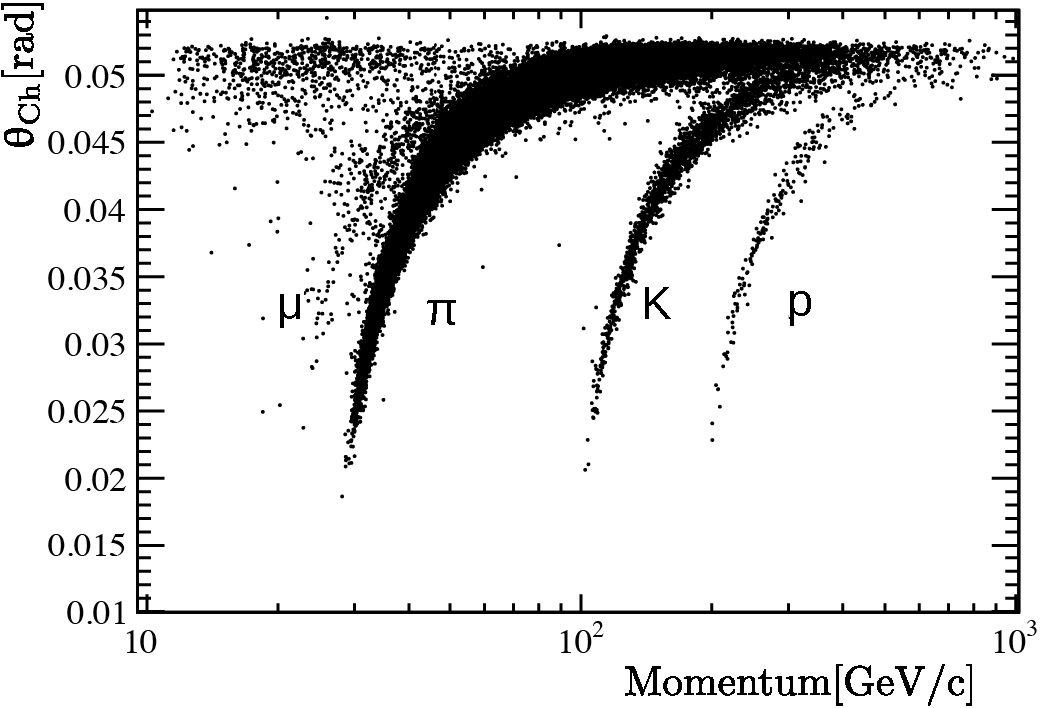
\includegraphics[width=0.75\textwidth]{figs/Method/ThetaVsMomentum_C4F10}
  \vspace{-0.5\baselineskip}
  \caption{
    Cherenkov angle \thetaC against track momentum, for tracks traversing the
    \richone gaseous radiator. Muons, pions, kaons and protons are visible. As
    the track momentum  increases, all particles tend towards the same \thetaC,
    known as the saturated Cherenkov angle.}
  \label{fig:saturation}
  \vspace{-0.5\baselineskip}
\end{figure}
For an aligned system position the mode of the \deltatheta distribution is
constant with $\phi$ for any mirror combination. It can be seen from
\fig{fig:RICH_MisalignmentDiagrams} (b), that any small  misalignment results in
an approximately sinusoidal dependence of the mode of the \deltatheta vs. $\phi$
distribution (described by Equation~\ref{eq:DeltaTheta_ps}).

Theoretically, to associate a ``Cherenkov angle" with a photon hit on the
photodetector plane, we need to ``reconstruct'' the photon, i.e. to
appropriately connect its point of emission, via two reflections, with the given
hit. The point of emission is certainly known only in MC. Because a photon
emitted from any point along the track (at the given $\phi$) will ideally hit
the same spot on the photodetector plane, in the case of data the emission point
should be chosen voluntarily. Analysis of MC events has
shown~\cite{Gorisek:1999td} that to reduce noise from the photons falsely
associated with a given track, only ``unambiguous" hits should be chosen. An
``unambiguous" hit yields reflection of the corresponding hypothetical photon
off the same combination of mirrors even if assumed to be emitted at the
beginning and at the end of the track path in the radiator. In our analysis we
use ``unambiguous" photons.

Our aim is to detect any extra rotations of all mirror segments, both primary
and secondary, around $z$ and $y$ axes against their position descriptions
contained in the Detector Description Database (DDDB) that had been already
corrected with the up-to-this-time misalignment corrections contained in the
Conditions Database (CONDDB).

Traditionally, all distances (displacements) on the photodetector plane are
expressed in terms of the polar angle $\theta$, which is approximately correct,
because optical paths for photons from the surface of a primary mirror to their
hits in the vicinity of the respective ring on the photodetector plane (for the
corresponding track and particular mirror combination, of course) are almost the
same.

As follows from \fig{fig:RICH_MisalignmentDiagrams}, if one or both of a
combination of primary mirror $p$ and secondary mirror $s$ are  misaligned, the
measured Cherenkov angle depends on $\phi$, and the difference between measured
and expected values looks like
\begin{equation}
  \label{eq:DeltaTheta_ps}
  \begin{aligned}
    \delta \theta_{p,s} (\phi) & \equiv   [\theta(\phi)-\theta_{\mathrm{Ch}} ]_{p,s}
                                 \approx  [\varTheta\cos(\phi-\varPhi)       ]_{p,s} \\
                               & =        [\varTheta\cos\varPhi\cos\phi
                                 +         \varTheta\sin\varPhi\sin\phi      ]_{p,s} \\
                               & =         \varTheta^z_{p,s}\cos\phi
                                 +         \varTheta^y_{p,s}\sin\phi                 \\
  \end{aligned}
\end{equation}
where $\varTheta^z_{p,s}$ and $\varTheta^y_{p,s}$ are combined tilts around
respective axes, resulting from tilts of both mirrors of the combination. On the
other hand, they are equal to the sum of those tilts taken with the so-called
``magnification factors''. Namely, the resulting displacement components of a
ring of photons reflected off a combination of primary mirror $p$ and secondary
mirror $s$, that are rotated by angles $\alpha^y_p$, $\alpha^z_p$, $\beta^y_s$
and $\beta^z_s$, respectively, are
\begin{equation}
  \label{eq:theta0_y_z}
  \begin{aligned}
      A^y_{p,s}\alpha^y_p+B^y_{p,s}\beta^y_s
    + a^y_{p,s}\alpha^z_p+b^y_{p,s}\beta^z_s & = \varTheta^y_{p,s} \\
      A^z_{p,s}\alpha^z_p+B^z_{p,s}\beta^z_s
    + a^z_{p,s}\alpha^y_p+b^z_{p,s}\beta^y_s & = \varTheta^z_{p,s}
  \end{aligned}
\end{equation}
where $A^y_{p,s}$, $B^y_{p,s}$, $a^y_{p,s}$ and $b^y_{p,s}$ ($A^z_{p,s}$,
$B^z_{p,s}$, $a^z_{p,s}$ and $b^z_{p,s}$ for the $z$-axis) are the corresponding
magnification factors, discussed in the next section.

To correct for the mirror misalignments, the projected combined mirror
misalignment onto the photodetector plane, $\varTheta^y_{p,s}$ and
$\varTheta^z_{p,s}$ in \fig{fig:RICH_MisalignmentDiagrams}, are determined for
each mirror combination from a subset of all possible mirror combinations
sufficient for determining misalignments of every mirror. This is achieved by
plotting $\delta\theta(\phi)_{p,s}$ and fitting it by a sinusoidal function (see
Equation~\ref{eq:DeltaTheta_ps}) as described in~\sect{subsec:Fitting}. This
misalignment is decomposed into a combination of individual primary and/or
secondary mirror rotational misalignments, as described
in~\sect{subsec:IndivMirrAlign}, by solving a system of linear equations,
similar to Equations~\ref{eq:theta0_y_z}. We correct for the misalignment by
applying corresponding compensating rotations to the mirrors. This procedure is
repeated until all the calculated remaining misalignments, $\alpha^y_p$,
$\alpha^z_p$, $\beta^y_s$ and $\beta^z_s$, are less than $0.1\mrad$.


\subsection{Magnification factors}
\label{subsec:Magnification}

To understand the origin of the magnification factors, let us consider in more
detail (although in simplified manner) how tilts of mirror segments affect
displacement of the Cherenkov ring against its expected position. For example,
small rotations of primary and secondary mirrors around their vertical ($y$)
axes yield approximately the following displacement of the ring in terms of
distance (note that rotation of a mirror by e.g. $\alpha^y$, results in
deflecting photons by $2\,\alpha^y$ in horizontal plane, as shown
in~\fig{fig:RICH_MisalignmentDiagrams}):
\begin{align*}
l\,\varTheta^y & \approx l_{\mathrm{pri}}2\,\alpha^y
                       - l_{\mathrm{sec}}2\, \beta^y,
\end{align*}
where $l$, $l_{\mathrm{pri}}$ and $l_{\mathrm{sec}}$ are paths of the photons to
the photodetectors (total, from primary, and from secondary mirrors,
respectively). Or in terms of Cherenkov angles

\begin{equation*}
  \varTheta^y  \approx \dfrac{2\,l_{\mathrm{pri}}}{l}\alpha^y
                     - \dfrac{2\,l_{\mathrm{sec}}}{l} \beta^y
               \approx                            A^y\alpha^y
                                                + B^y \beta^y.
\end{equation*}
Similarly, for small rotations around horizontal axes
\begin{equation*}
\varTheta^z  \approx \dfrac{2\,l_{\mathrm{pri}}}{l}\alpha^z
                   + \dfrac{2\,l_{\mathrm{sec}}}{l} \beta^z
             \approx                            A^z\alpha^z
                                              + B^z \beta^z.
\end{equation*}
For each mirror combination the magnification factors are evaluated by
introducing 8 independent calibrational rotations (positive or negative
rotations about the $y-$ or $z-$axes for the primary or secondary mirrors) and
by measuring the resulting total tilts. In particular, $\pm0.3\mrad$ rotations
are used. That choice is motivated by the fact that typically, Cherenkov angle
resolution, the half-width of the $\theta$ distribution, for \richtwo is around
$0.7\mrad$. The final value of each factor is arithmetical mean of the two
corresponding values obtained with the calibrating rotations in opposite
directions.

Although na\"{\i}vely we would expect $l=l_{\mathrm{pri}}$, in practice, due to
complicated averaging of the ``reconstructed'' photon paths for every mirror
combination, the factors have somewhat differing values, and on average look
approximately like
\begin{equation*}
  \varTheta^y  \approx 2.0\,\alpha^y-0.9\,\beta^y
  \;\;\text{and}\;\;
  \varTheta^z  \approx 1.8\,\alpha^z+0.6\,\beta^z.
\end{equation*}
In reality, there is also a small but still significant cross-influence between
rotations around alternative axes: e.g. rotation of a mirror around $y$-axis
yields also a small deflection of the photon in the perpendicular plane, i.e.
around $z$-axis. That is why Equations~\ref{eq:theta0_y_z}
contain also the corresponding cross-terms. As for the cross-term magnification
factors, $a^y,\;b^y,\;a^z\;\text{and}\;b^z$, their absolute values vary
approximately between 0.001 and 0.250, and they can be positive as well as
negative.


\subsection{Alignment parameters}

A list of alignment parameters is shown in \tab{tab:AlignmentParameters}. The
table outlines the parameters which are observable and those that need to be
found and corrected for in the alignment process.
\begin{table}[htb]
  \vspace{-0.5\baselineskip}
  \caption{
    Alignment parameters.}
  \vspace{-0.5\baselineskip}
  \centering
  \begin{longtable}{c p{0.8\textwidth}}
    Parameter                               & \multicolumn{1}{c}{Definition} \\
    \midrule
    $p$                                     & primary   mirror number: 0-3  for \richone, 0-55 for \richtwo\\
    $s$                                     & secondary mirror number: 0-15 for \richone, 0-39 for \richtwo\\
    $\varTheta^y_{p,s}$/$\varTheta^z_{p,s}$ & observed combined misalignment on the photo-detector plane in the $y$-axis/$z$-axis, for mirror combination $(p,s)$\\
    $\alpha^y_p$/$\alpha^z_p$               & calculated misalignment of primary   mirror $p$ as a tilt about its local $y$-axis/$z$-axis\\
    $ \beta^y_s$/$ \beta^z_s$               & calculated misalignment of secondary mirror $s$ as a tilt about its local $y$-axis/$z$-axis\\
    $A^y_{p,s}$/$A^z_{p,s}$                 & magnification factor to map $\alpha^y_p$/$\alpha^z_p$ onto $\varTheta^y_{p,s}$/$\varTheta^z_{p,s}$ (tilts resulting from rotations around the same axes)\\
    $B^y_{p,s}$/$B^z_{p,s}$                 & magnification factor to map $ \beta^y_s$/$ \beta^z_s$ onto $\varTheta^y_{p,s}$/$\varTheta^z_{p,s}$ (tilts resulting from rotations around the same axes)\\
    $a^y_{p,s}$/$a^z_{p,s}$                 & magnification factor to map $\alpha^z_p$/$\alpha^y_p$ onto $\varTheta^y_{p,s}$/$\varTheta^z_{p,s}$ (minor tilts resulting from rotations around the alternative axes)\\
    $b^y_{p,s}$/$b^z_{p,s}$                 & magnification factor to map $ \beta^z_s$/$ \beta^y_s$ onto $\varTheta^y_{p,s}$/$\varTheta^z_{p,s}$ (minor tilts resulting from rotations around the alternative axes)\\
  \end{longtable}
  \label{tab:AlignmentParameters}
  \vspace{-0.5\baselineskip}
\end{table}
Note that the magnification factors are not
known in advance and need to be found as well, as was discussed
in~\sect{subsec:Magnification}.


\subsection{Fitting method}
\label{subsec:Fitting}

For every chosen combination of primary mirror $p$ and secondary mirror $s$,
\deltatheta is plotted against $\phi$. Each of these histograms is divided into
20 bins in $\phi$. Inside each $\phi$ bin the \deltatheta distribution is fitted
with a Gaussian plus first/second order (for \richone/\richtwo) polynomial
background. In accordance with Equation~\ref{eq:DeltaTheta_ps} the $\phi$
dependence of the position of the Gaussian peak for a given mirror combination
$(p,s)$ is approximated by
\begin{equation}
  \label{eq:Delta_theta}
  \delta\theta_{p,s}(\phi) = \varTheta^z_{p,s}\cos\phi
                           + \varTheta^y_{p,s}\sin\phi.
\end{equation}
Equation~\ref{eq:Delta_theta} is used as a bond when fitting all the 20 slices
jointly. The fitting is done by means of the \root
framework~\cite{Antcheva:2011zz}, in particular, using the \minuit2 minimization
package. The values of the fitted parameters $\varTheta^y_{p,s}$ and
$\varTheta^z_{p,s}$ correspond to misalignment of that mirror combination mapped
to apparent displacement of the ring on the photodetector plane, as explained in
\fig{fig:RICH_MisalignmentDiagrams}. An example of such a fit for misaligned
mirror combination $(0,1)$ of \richone is shown in
\fig{fig:Rich1Mirr0001dThetavphiRec}: before alignment (left), and after
alignment (right).
\begin{figure}[htbp]
  \vspace{-0.5\baselineskip}
  \centering
  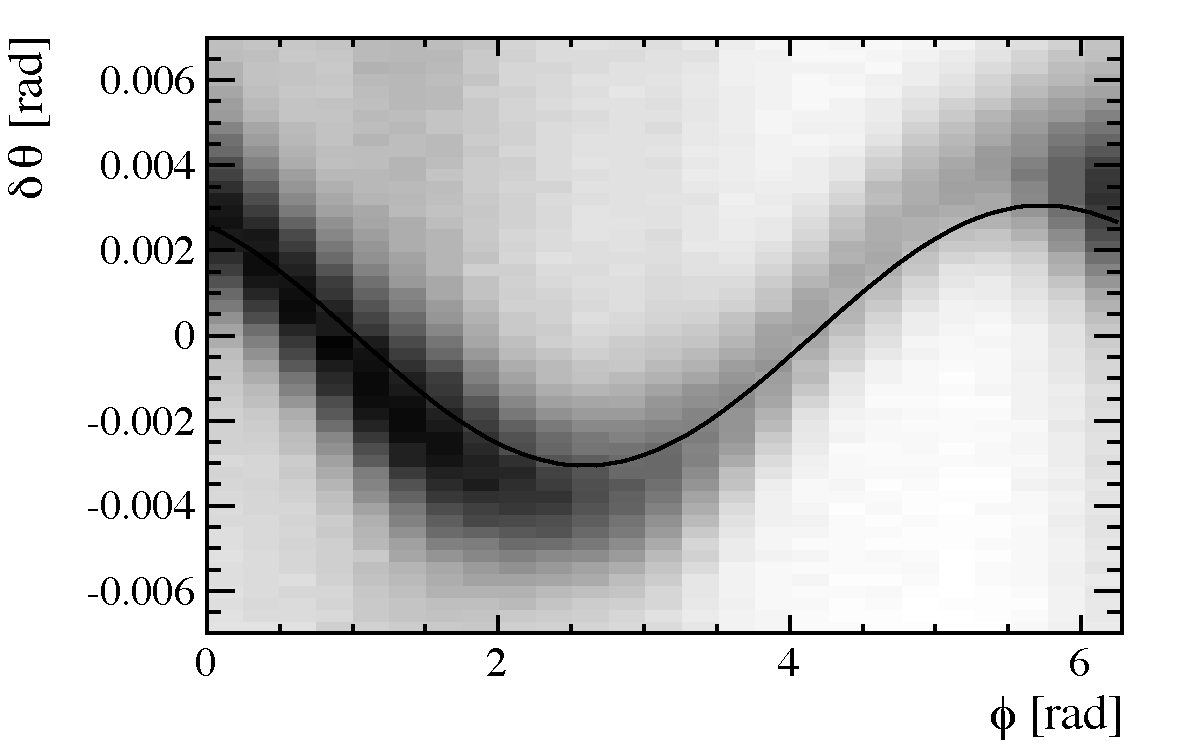
\includegraphics[width=.49\textwidth]
    {figs/Method/RICH1_ThetaVsPhiRec0001_misaligned.pdf}
  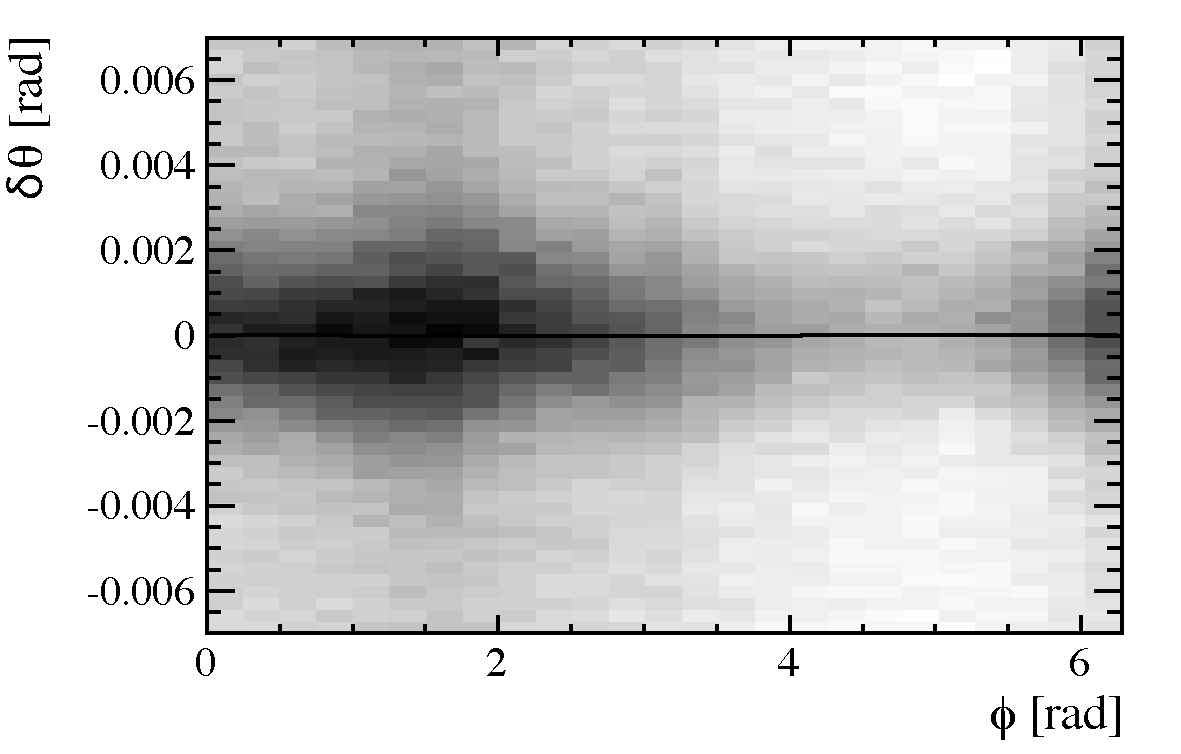
\includegraphics[width=.49\textwidth]
    {figs/Method/RICH1_ThetaVsPhiRec0001_aligned.pdf}
  \vspace{-1.0\baselineskip}
  \caption{
    \deltatheta against $\phi$ fitted slice-by-slice along $\phi$ with
    function~\eqref{eq:Delta_theta} approximating position of the Gaussian peak
    on the $\phi\text{-}\delta\theta$~plane for combination of primary mirror 0
    and secondary mirror 1 of \richone detector. The originally misaligned
    mirror combination is represented on the left. On the right --- same fit
    after the combination is aligned.}
  \label{fig:Rich1Mirr0001dThetavphiRec}
  \vspace{-0.5\baselineskip}
\end{figure}


\subsection{Determining individual mirror misalignments}
\label{subsec:IndivMirrAlign}

If we can map a measured Cherenkov ring misalignment to individual mirror
rotations, we can compensate for it in the software. Obviously, there is no
straightforward way to do that. However, optimal alignment can be achieved if
each component of the optical system is properly aligned relative to all others.
In this sense finding the absolute alignment of each individual component is not
significantly important. We therefore aim to align all mirrors relative to each
other.


\subsubsection{\richone alignment}
\label{subsec:Rich1Align}


The geometry of the \lhcb \richone detector restricts the number of populated
mirror combinations to 16, \fig{fig:RICH1_MirrorNumbering}. Photons reflected
off a primary mirror are then reflected off one of four secondary mirrors that
form a group, unique to that primary mirror. Each of the four quadrants contain
a single primary mirror and four secondary mirrors. The misalignments of the
four mirror combinations in each quadrant are determined using the method
discussed in~\sect{subsec:Fitting}.
\begin{figure}[htbp]
  \vspace{-0.5\baselineskip}
  \centering
  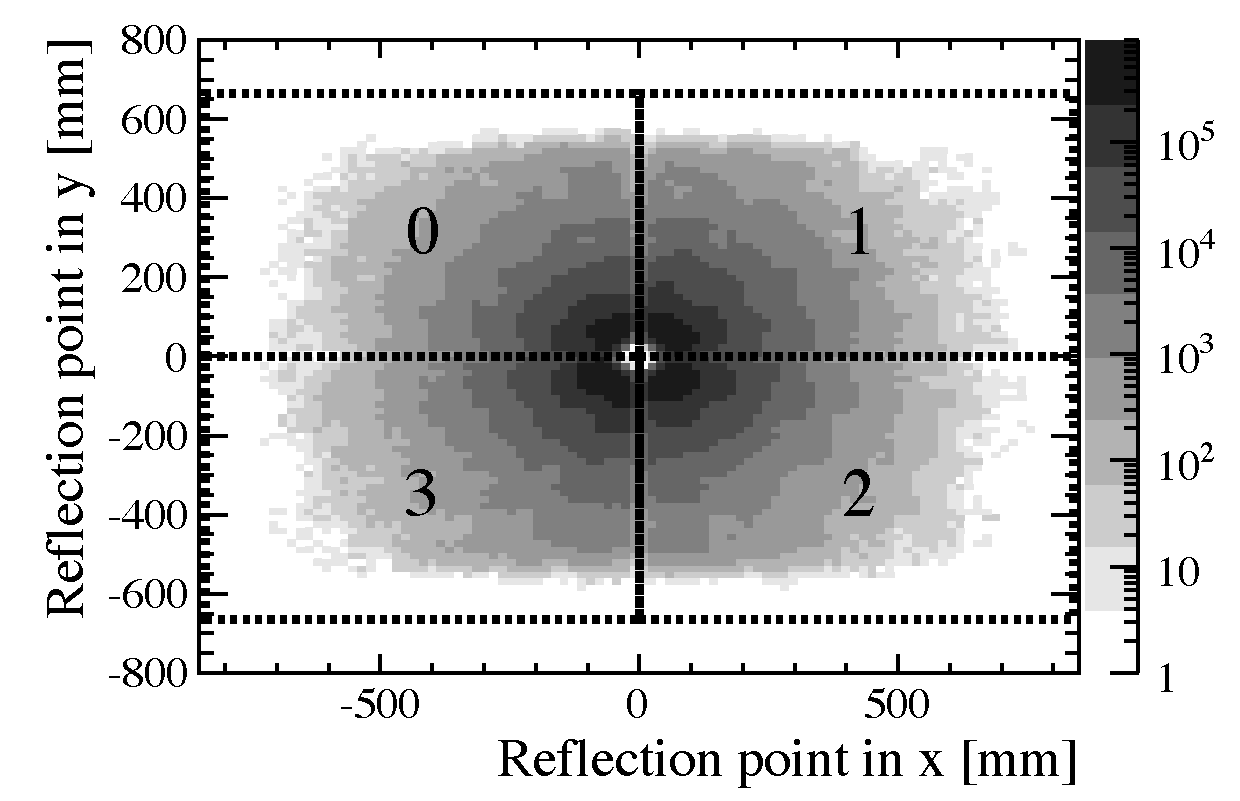
\includegraphics[width=.48\textwidth]{figs/Method/RICH1_PrimaryMirrors.pdf}
  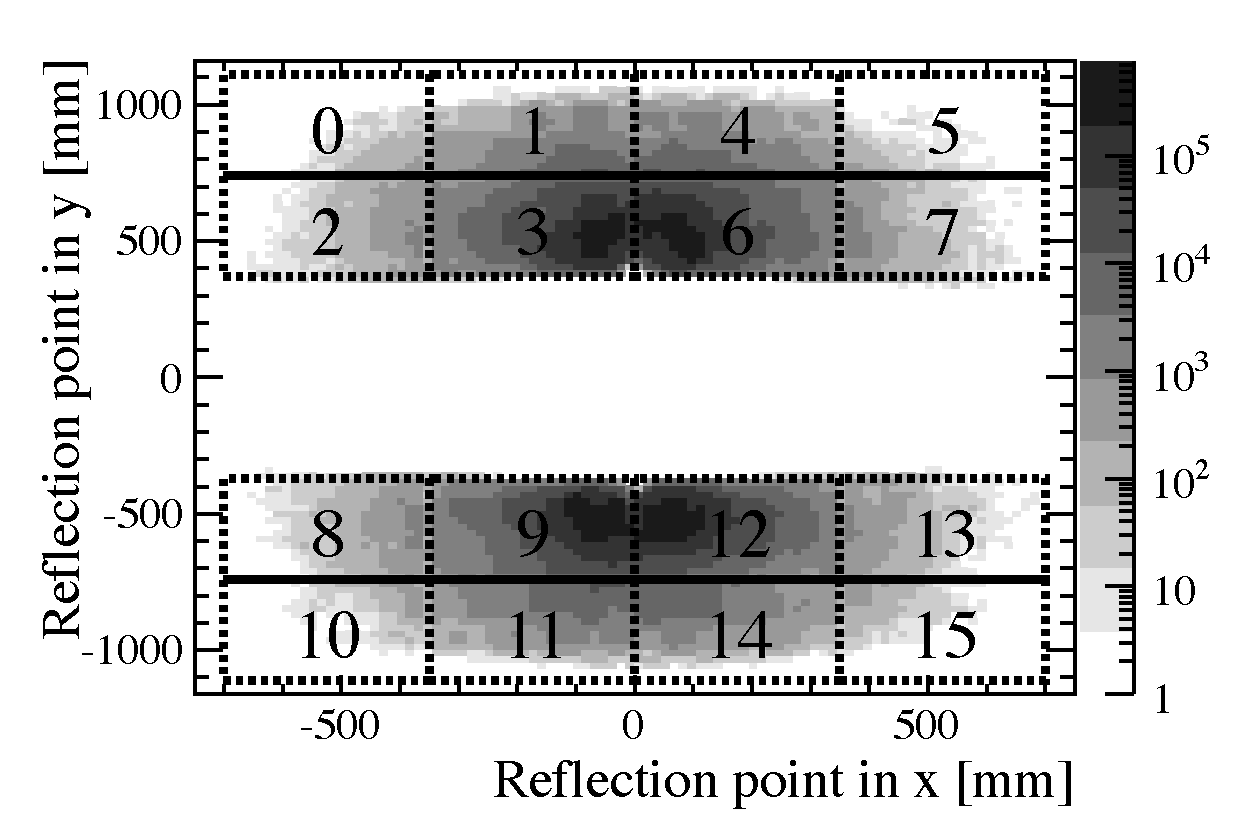
\includegraphics[width=.48\textwidth]{figs/Method/RICH1_SecondaryMirrors.pdf}
  \vspace{-0.5\baselineskip}
  \caption{
    Reflection point distribution of photons off \richone primary mirrors (left)
    and secondary mirrors (right). The photon population across mirrors is not
    uniform with the higher populated mirrors laying closest to the beam-pipe.
    Also shown is the \richone mirror numbering schema, viewed along the beam.}
  \label{fig:RICH1_MirrorNumbering}
  \vspace{-0.5\baselineskip}
\end{figure}

Thus, e.g. for quadrant 0 in the $y$-direction, we have four equations for five
unknowns ($\alpha^{y}_{0},\beta^{y}_{0},\dotsc,\beta^{y}_{3}$)
\begin{equation*}
  \label{eq:zeroQuadrantMirrorTilts}
  \arraycolsep=1pt
  \begin{array}{*{5}c}
    A^y_{0,0}\alpha^y_0 & + & B^y_{0,0}\beta^y_0 & = & \varTheta^y_{0,0} \\
    \vdots              &   & \vdots             &   & \vdots \\
    A^y_{0,3}\alpha^y_0 & + & B^y_{0,3}\beta^y_3 & = & \varTheta^y_{0,3}.
  \end{array}
\end{equation*}
One option is to exclude the primary mirror from the adjustment procedure, i.e.
set $\alpha^y_0=0$, and then directly calculate misalignments of each secondary
mirror: $\beta^y_s=\varTheta^y_{0,s}/B^y_{0,s}$.

Instead, we first attempt to align the primary mirrors. For each quadrant, we
temporarily neglect misalignments of the secondary mirrors, i.e. set
$\beta^y_s=0$, calculate four misalignment estimates $(\alpha^y_p)_s =
\varTheta^y_{p,s}/A^y_{p,s}$ for the primary mirror (in conjunction with the
four different secondary mirrors $s$) and their average
\begin{equation*}
  \alpha^y_p = \frac{1}{4} \displaystyle\sum\limits_s(\alpha^y_p)_s
\end{equation*}
becomes an estimate of misalignment of that primary mirror. It is then
used to find the misalignment of each secondary mirror of that quadrant:
\begin{equation*}
  \beta^y_s = \frac{\left(\varTheta^y_{p,s} - A^y_{p,s}\alpha^y_p\right)}
                   {B^y_{p,s}}.
\end{equation*}
The final effect of the misalignment compensation is the same as in case of the
first option, although the individual mirror adjustments are different. All the
obtained adjustments are then inserted into the software. The same is done for
misalignments around the $z$-axis.

Because the magnification factors become slightly altered after the mirror
adjustment, we are unable to find the final solution of the system of equations
in one pass. Therefore, we iterate over the same data --- re-evaluating the
total tilts produced by each combination and the respective magnification
factors using the updated compensations --- until the calculated remaining
misalignments, $\alpha^y_p$, $\alpha^z_p$, $\beta^y_s$ and $\beta^z_s$, are less
than $0.1\mrad$.


\subsubsection{\richtwo alignment}

The geometrical layout of the \richtwo detector is significantly different to
that of \richone, and therefore we cannot find the mirror misalignments with
the same method.

The \richtwo detector has 56 primary (mostly hexagonal) and 40 secondary
(rectangular) mirror segments. Each hexagonal segment can be inscribed in a
circle of a radius of $r_{\mathrm{m}} = 251\mm$. The maximum base radius of the
Cherenkov cones on the primary mirrors is $r_{\mathrm{Ch}} = 55\mm$, therefore
probability of having a ring imaged by only one primary mirror segment is
$p_{\mathrm{Ch}} \approx 1 - r_{\mathrm{Ch}}/r_{\mathrm{m}} \approx 78\%$, which
makes easier pattern recognition and correction in case of mirror
misalignments~\cite{D'Ambrosio:2001ooa}.

All mirrors are divided into two decoupled systems: 48 on the left of the beam,
and 48 on the right of the beam. This gives 96 unknown parameters for each side
(tilts around $y$ and $z$ axes for each mirror). Their numbering schema is shown
in~\fig{fig:RICH2_MirrorNumbering}
\begin{figure}[htbp]
  \vspace{-0.5\baselineskip}
  \centering
  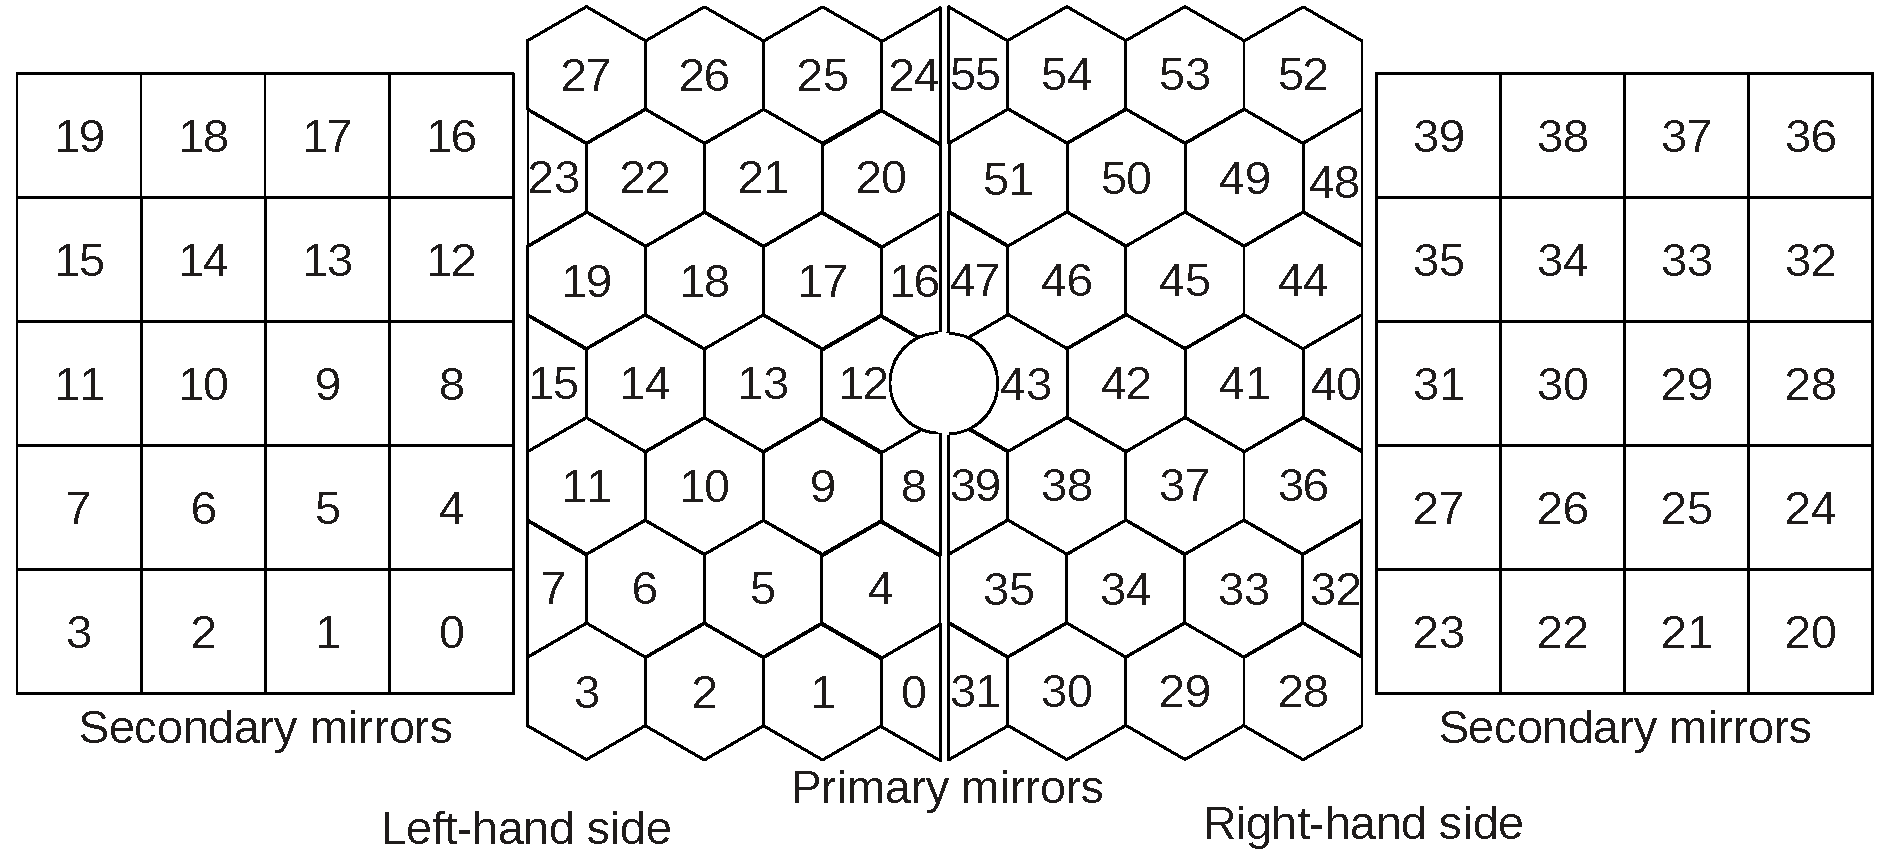
\includegraphics[width=\textwidth]{figs/Method/RICH2_MirrorNumberingBothSides.pdf}
  \vspace{-1.0\baselineskip}
  \caption{
    \richtwo mirror segmentation and the numbering schema, viewed
    along the beam. The beampipe is at the centre.}
  \label{fig:RICH2_MirrorNumbering}
  \vspace{-0.5\baselineskip}
\end{figure}

However, only 47 out of 48 possible tilts around each axis are independent,
because if we simultaneously rotate all primary mirrors by one angle and all
secondary mirrors by the corresponding angle in the opposite direction, the ring
position will not change.

%\setlength{\tabcolsep}{0pt}
%\begin{table}[htb]
%  \caption{
%    Chosen  47 $p,s$ (primary,secondary) mirror combinations (left-hand side of
%    \richtwo). Vertical axis presents primary mirror numbers, horizontal ---
%    secondary.}
%  \vspace{-0.5\baselineskip}
%  \tiny
%  \sffamily
%  \begin{tabular}{ c | *{20}{ >{\centering}p{0.048\textwidth} } }
%       &     0 &     1 &     2 &     3 &     4 &     5 &     6 &     7 &     8 &     9 &    10 &    11 &    12 &    13 &    14 &    15 &    16 &    17 &    18 &    19 \tabularnewline
%    \hline
%     0 &   0,0 &       &       &       &       &       &       &       &       &       &       &       &       &       &       &       &       &       &       &       \tabularnewline
%     1 &       &   1,1 &       &       &       &       &       &       &       &       &       &       &       &       &       &       &       &       &       &       \tabularnewline
%     2 &       &       &   2,2 &       &       &       &       &       &       &       &       &       &       &       &       &       &       &       &       &       \tabularnewline
%     3 &       &       &       &   3,3 &       &       &       &       &       &       &       &       &       &       &       &       &       &       &       &       \tabularnewline
%     4 &   4,0 &   4,1 &       &       &       &   4,5 &       &       &       &       &       &       &       &       &       &       &       &       &       &       \tabularnewline
%     5 &       &       &   5,2 &       &       &       &   5,6 &       &       &       &       &       &       &       &       &       &       &       &       &       \tabularnewline
%     6 &       &       &       &   6,3 &       &       &       &   6,7 &       &       &       &       &       &       &       &       &       &       &       &       \tabularnewline
%     7 &       &       &       &       &       &       &       &   7,7 &       &       &       &       &       &       &       &       &       &       &       &       \tabularnewline
%     8 &       &       &       &       &   8,4 &       &       &       &   8,8 &       &       &       &       &       &       &       &       &       &       &       \tabularnewline
%     9 &       &       &       &       &       &   9,5 &       &       &       &   9,9 &       &       &       &       &       &       &       &       &       &       \tabularnewline
%    10 &       &       &       &       &       &       &  10,6 &       &       &       & 10,10 &       &       &       &       &       &       &       &       &       \tabularnewline
%    11 &       &       &       &       &       &       &       &  11,7 &       &       &       & 11,11 &       &       &       &       &       &       &       &       \tabularnewline
%    12 &       &       &       &       &       &       &       &       &  12,8 &  12,9 &       &       &       &       &       &       &       &       &       &       \tabularnewline
%    13 &       &       &       &       &       &       &       &       &       &  13,9 & 13,10 &       &       &       &       &       &       &       &       &       \tabularnewline
%    14 &       &       &       &       &       &       &       &       &       &       & 14,10 & 14,11 &       &       &       &       &       &       &       &       \tabularnewline
%    15 &       &       &       &       &       &       &       &       &       &       &       & 15,11 &       &       &       &       &       &       &       &       \tabularnewline
%    16 &       &       &       &       &       &       &       &       &  16,8 &       &       &       & 16,12 &       &       &       &       &       &       &       \tabularnewline
%    17 &       &       &       &       &       &       &       &       &       &  17,9 &       &       &       & 17,13 &       &       &       &       &       &       \tabularnewline
%    18 &       &       &       &       &       &       &       &       &       &       & 18,10 &       &       &       & 18,14 &       &       &       &       &       \tabularnewline
%    19 &       &       &       &       &       &       &       &       &       &       &       & 19,11 &       &       &       & 19,15 &       &       &       &       \tabularnewline
%    20 &       &       &       &       &       &       &       &       &       &       &       &       &       & 20,13 &       &       & 20,16 & 20,17 &       &       \tabularnewline
%    21 &       &       &       &       &       &       &       &       &       &       &       &       &       &       & 21,14 &       &       &       & 21,18 &       \tabularnewline
%    22 &       &       &       &       &       &       &       &       &       &       &       &       &       &       &       & 22,15 &       &       &       & 22,19 \tabularnewline
%    23 &       &       &       &       &       &       &       &       &       &       &       &       &       &       &       & 23,15 &       &       &       &       \tabularnewline
%    24 &       &       &       &       &       &       &       &       &       &       &       &       &       &       &       &       & 24,16 &       &       &       \tabularnewline
%    25 &       &       &       &       &       &       &       &       &       &       &       &       &       &       &       &       &       & 25,17 &       &       \tabularnewline
%    26 &       &       &       &       &       &       &       &       &       &       &       &       &       &       &       &       &       &       & 26,18 &       \tabularnewline
%    27 &       &       &       &       &       &       &       &       &       &       &       &       &       &       &       &       &       &       &       & 27,19 \tabularnewline
%  \end{tabular}
%  \label{tab:ChosenConbinationsDiagonal}
%  \vspace{-0.5\baselineskip}
%\end{table}

\setlength{\tabcolsep}{6pt}
\newcolumntype{d}[1]{ D{,} {,} {#1} }

\begin{table}[htb]
  \caption{
    Chosen 47 $p,s$ (primary,secondary) mirror combinations grouped by primary mirror
    numbers (left-hand side of \richtwo).}
  \vspace{-0.5\baselineskip}
  \centering
 %\scriptsize
  \small
  \sffamily
  \begin{tabular}{*{4}{|d{2}d{2}}|}
    \hline
           & 27,19 &       & 26,18 &       & 25,17 &       & 24,16 \\
    \hline
           &       & 22,19 & 22,18 &       & 21,17 &       & 20,16 \\
           & 23,15 &       & 22,14 &       & 21,13 &       & 20,12 \\
    \hline
           & 19,15 &       & 18,14 &       & 17,13 &       & 16,12 \\
           & 19,11 &       & 18,10 &       & 17,9  &       & 16,8  \\
    \hline
           & 15,11 & 14,11 & 14,10 & 13,10 & 13,9  & 12,9  & 12,8  \\
    \hline
           & 11,11 &       & 10,10 &       &  9,9  &       &  8,8  \\
           & 11,7  &       & 10,6  &       &  9,5  &       &  8,4  \\
    \hline
           &  7,7  &       &  6,6  &       &  5,5  &       &  4,4  \\
           &       &  6,3  &  6,2  &       &  5,1  &       &  4,0  \\
    \hline
           &  3,3  &       &  2,2  &       &  1,1  &       &  0,0  \\
    \hline
  \end{tabular}
  \label{tab:ChosenConbinationsPri}
  \vspace{-0.5\baselineskip}
\end{table}

\begin{table}[htb]
  \caption{
    Chosen 47 $p,s$ (primary,secondary) mirror combinations grouped by secondary mirror
    numbers (left-hand side of \richtwo).}
  \vspace{-0.5\baselineskip}
  \centering
 %\scriptsize
  \small
  \sffamily
  \begin{tabular}{*{4}{|d{2}d{2}}|}
    \hline
           & 27,19 &       & 26,18 &       & 25,17 &       & 24,16 \\
           & 22,19 &       & 22,18 &       & 21,17 &       & 20,16 \\
    \hline
           & 23,15 &       & 22,14 &       & 21,13 &       & 20,12 \\
           & 19,15 &       & 18,14 &       & 17,13 &       & 16,12 \\
    \hline
           & 19,11 &       & 18,10 &       & 17,9  &       & 16,8  \\
     15,11 & 14,11 & 14,10 & 13,10 & 13,9  & 12,9  &       & 12,8  \\
           & 11,11 &       & 10,10 &       &  9,9  &       &  8,8  \\
    \hline
           & 11,7  &       & 10,6  &       &  9,5  &       &  8,4  \\
           &  7,7  &       &  6,6  &       &  5,5  &       &  4,4  \\
    \hline
           &  6,3  &       &  6,2  &       &  5,1  &       &  4,0  \\
           &  3,3  &       &  2,2  &       &  1,1  &       &  0,0  \\
    \hline
  \end{tabular}
  \label{tab:ChosenConbinationsSec}
  \vspace{-0.5\baselineskip}
\end{table}

%Tables~\ref{tab:ChosenConbinationsDiagonal},~\ref{tab:ChosenConbinationsPri}
%and~\ref{tab:ChosenConbinationsSec}~--
%
%Table~\ref{tab:ChosenConbinationsPri} and~\fig{fig:RICH2_MirrCombinSchema}~--
%
Tables~\ref{tab:ChosenConbinationsPri} and~\ref{tab:ChosenConbinationsSec}
and~\fig{fig:RICH2_MirrCombinSchema}~--
%
each in its own way~-- present the set of combinations chosen for the alignment
procedure. The goal is to have consistent system of equations for determining
the individual misalignments. In particular, it is seen, that almost each
primary mirror is combined with at least two secondary mirrors. Overall, useful
mirror combinations are selected such that all mirrors are linked together. By
fixing the misalignment of one of the primary mirrors (12) we find the
misalignment of the secondary mirror with which it forms a combination. This
secondary mirror also forms combination with another primary mirror which allows
to find its misalignment in turn. This linking continues until all mirrors in
each side of \richtwo are related.
\begin{figure}[htbp]
  \vspace{-0.5\baselineskip}
  \centering
  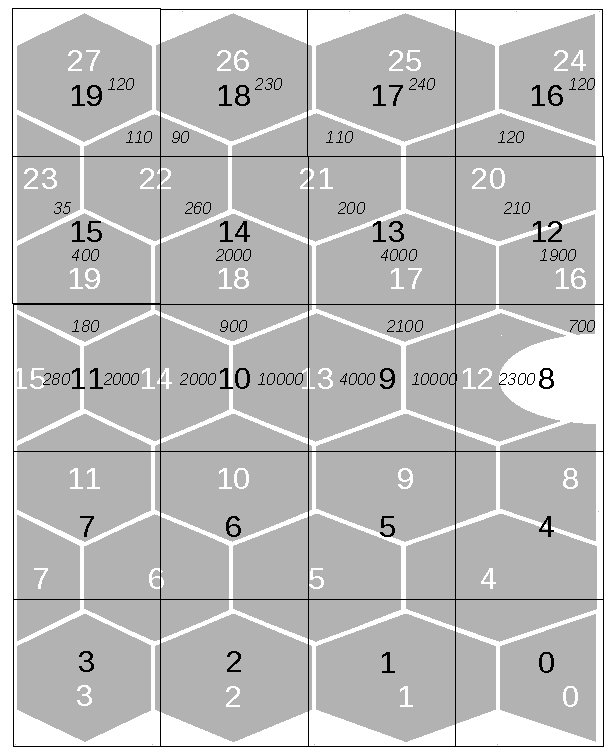
\includegraphics[width=0.6\textwidth]{figs/Method/RICH2_MirrCombins_numbersAfterSelection.pdf}
  \vspace{-0.4\baselineskip}
  \caption{
    \richtwo (left-hand side) primary/secondary mirror optical overlapping and
    the optimal combining schema based on the results of the selection
    (Section~\ref{sec:SelectionMethod}). Black transparent square boxes with
    black numbers~-- secondary mirrors, gray hexagons or trapezoids with white
    numbers~-- primary ones. The relative population numbers of the mirror
    combination histograms, taken from~\fig{fig:mirrPopsSelected}, are
    multiplied by $10^4$. The system of equations~\ref{eq:theta0_y_z} follows
    this optimal overlapping schema.}
  \label{fig:RICH2_MirrCombinSchema}
  \vspace{-0.6\baselineskip}
\end{figure}

Consistent set of combinations is not unique. So we have chosen the set with
maximal populated combinations. That choice can be read
off~\fig{fig:mirrPopsSelected}.

Next we need a system of equations for finding these parameters. Each equation
will represent a combination of one primary and one secondary mirror segment. In
reality, the number of these equations hardly reaches the number of the
unknowns, because each mirror ``collaborates'' efficiently (in terms of
reflecting the same photons) with not more than a couple of other adjacent
mirrors of the opposite kind. From the point of view of geometrical optics, this
means that a set of small rotations of one kind of mirrors can be approximately
compensated by a set of small rotations of mirrors of the opposite kind in the
compensating directions, so that nothing changes on the photo-detector plane.
Therefore, a formally consistent system of 96 equations relating tilts around
$y$ and $z$ axes for 28 primary and 20 secondary mirrors will be
ill-conditioned, meaning that although there will always exist a formally unique
solution, in practice it will be unstable. That instability will reveal itself
in non-convergence of the solutions, because the magnification factors and the
``measured'' combined tilts for each combination will slightly variate from
iteration to iteration, and although the system will be numerically close to the
previous one, it will yield a somewhat different solution which will, in turn,
result in a next fluctuation of the system, preventing further adjustments from
reaching desired smallness.

The most straightforward way to regularize the solution is simply to give up
adjusting one of the mirrors, fixing its adjustments to 0. We have chosen
primary mirror 12 for that. This is because of its relatively high photon
population, being the closest mirror to the beam pipe.

Among all possible mirror combinations we have consistently chosen first 47
combinations from their list sorted according to their efficiency in jointly
reflecting photons in descending order. This choice is shown in
Table~\ref{tab:ChosenConbinationsPri} and~\fig{fig:RICH2_MirrCombinSchema}.

As a result, we have a system of 94 linear equations (47 combinations of
Equations~\ref{eq:theta0_y_z}). We solve this system algebraically, by the
substitution method at the combinations level (starting with setting tilts of
primary mirror 12 equal to zero: $\alpha^y_{12}=\alpha^z_{12}=0$) and with
Cramer's rule --- within each combination (system of
equations~\ref{eq:theta0_y_z}).

Obviously, last paragraph of the previous section (\sect{subsec:Rich1Align})
applies here too.


\subsubsection{Improvement of the mathematical schema}

The above approach to solving the system of equations for compensations for the
individual mirror segment misalignments suffers from inequality: one mirror in
each set of mirrors that are treated jointly, is privileged and is not being
corrected at all. As it is pointed out above, this is because the whole
geometrical configuration of the mirror system is inherently degenerate
numerically.

In HERAb an attempt was implemented to solve the analogous system using least
squares method augmented by requirement that the algebraic sum of the
corrections (secondary mirror adjustments are included with the opposite sign)
is minimal, which gives them an additional equation that makes solution of the
system quasi unique~\cite{Staric:2007vf}. That system was solved by the weighted
least squares method with two caveats: a) only dispersions of the right-hand
sides were used and b) the weight for the squared discrepancy of the additional
equation was chosen rather voluntarily. Although that approach eliminated
privilege of one of the mirrors in each set, it is not satisfactory, and one of
the reasons is that the additional equation is only a linear sum, while there
should have been some sort of a quadratic sum.

We essentially improved the computations in the following way. Let us first
consider general case and then translate the formulae to our specific notations.
Let the underdetermined system of $n-1$ equations for $n$ unknowns be
\begin{equation}
  \label{eq:GenericSystem}
  \arraycolsep=1pt
  \begin{array}{*{11}c}
     a_{1,1}x_1    &+& \cdots   &+& a_{1,k}x_k     &+& \cdots  &+& a_{1,n}x_n   &=& b_1        \\
     \vdots        & & \ddots   & & \vdots         & & \ddots  & & \vdots       & & \vdots     \\
     a_{n-1,1}x_1  &+& \cdots   &+& a_{n-1,k}x_k   &+& \cdots  &+& a_{n-1,n}x_n &=& b_{n-1}.
  \end{array}
\end{equation}
To get a unique solution we need, e.g., to determine one of the values, say
$x_k$, a priori, from a different source. Simplest way is to fix it as $x_k=0$.

Instead, we have chosen a more sophisticated method: we add a regularizing
constraint. Namely, we minimize the overall perturbation of the system, i.e.
minimize the Euclidean norm of the solution vector
\begin{equation}
  \label{eq:EuclideanNorm}
  \displaystyle\sum\limits_{j=1}^n x_j^2.
\end{equation}

Then, modified ``weighted'' least squares method will consist in minimizing the
following functional:
\begin{equation}
  \label{eq:LeastSquareSolution}
  \displaystyle\sum\limits_{j=1}^n
  \left[
  \displaystyle\sum\limits_{i=1}^{n-1}
          \frac{\bigg(    b_i  - \displaystyle\sum\limits_{j=1}^n         a_{i,j} x_j \bigg)^2}
               { \sigma^2(b_i) + \displaystyle\sum\limits_{j=1}^n\sigma^2(a_{i,j})x_j^2}
  + x_j^2
  \right]
  ,
\end{equation}.




while the in the ``unweighted'' case it becomes
\begin{equation}
  \label{eq:UnweightedLeastSquareSolution}
  \displaystyle\sum\limits_{j=1}^n
  \left[
  \displaystyle\sum\limits_{i=1}^{n-1}
          \bigg(          b_i  - \displaystyle\sum\limits_{j=1}^n         a_{i,j} x_j \bigg)^2
  + x_j^2
  \right]
  .
\end{equation}

 
In our particular case and with our specific notations (this is equally valid
for both \richone and \richtwo), instead of~\eqref{eq:GenericSystem}
and~\eqref{eq:LeastSquareSolution}, we have system of
equations~\eqref{eq:GenericSystemRICH}
\begin{equation}
  \label{eq:GenericSystemRICH}
  \arraycolsep=1pt
  \begin{array}{*{9}c}
%     A^y_{0,0}\alpha^y_0      &+& B^y_{0,0}\beta^y_0      &+& a^y_{0,0}\alpha^z_0      &+& b^y_{0,0}\beta^z_0      &=& \varTheta^y_{0,0}   \\
%     A^z_{0,0}\alpha^z_0      &+& B^z_{0,0}\beta^z_0      &+& a^z_{0,0}\alpha^y_0      &+& b^z_{0,0}\beta^y_0      &=& \varTheta^z_{0,0}   \\
      \vdots                   & & \vdots                  & & \vdots                   & & \vdots                  & & \vdots              \\
      A^y_{p,s}\alpha^y_{p}    &+& B^y_{p,s}\beta^y_s      &+& a^y_{p,s}\alpha^z_{p}    &+& b^y_{p,s}\beta^z_s      &=& \varTheta^y_{p,s}   \\
      A^z_{p,s}\alpha^z_{p}    &+& B^z_{p,s}\beta^z_s      &+& a^z_{p,s}\alpha^y_{p}    &+& b^z_{p,s}\beta^y_s      &=& \varTheta^z_{p,s}   \\
      \vdots                   & & \vdots                  & & \vdots                   & & \vdots                  & & \vdots              \\
%     A^y_{27,19}\alpha^y_{27} &+& B^y_{27,19}\beta^y_{19} &+& a^y_{27,19}\alpha^z_{27} &+& b^y_{27,19}\beta^z_{19} &=& \varTheta^y_{27,19} \\
%     A^z_{27,19}\alpha^z_{27} &+& B^z_{27,19}\beta^z_{19} &+& a^z_{27,19}\alpha^y_{27} &+& b^z_{27,19}\beta^y_{19} &=& \varTheta^z_{27,19} \\
  \end{array}
\end{equation}
and we would minimize functional~\eqref{eq:LeastSquareSolutionRICH},
respectively:
\begin{equation}
  \label{eq:LeastSquareSolutionRICH}
  \begin{aligned}
    \displaystyle\sum_{p,s \in \mathrm{subset}}
      \bigg[ 
             &  \frac{(\varTheta^y_{p,s}  -          A^y_{p,s}  \alpha^y_p
                                          -          B^y_{p,s}   \beta^y_s
                                          -          a^y_{p,s}  \alpha^z_p
                                          -          b^y_{p,s}   \beta^z_s)^2}
             {\sigma^2(\varTheta^y_{p,s}) + \sigma^2(A^y_{p,s})(\alpha^y_p)^2
                                          + \sigma^2(B^y_{p,s})( \beta^y_s)^2
                                          + \sigma^2(a^y_{p,s})(\alpha^z_p)^2
                                          + \sigma^2(b^y_{p,s})( \beta^z_s)^2} \\
           + &  \frac{(\varTheta^z_{p,s}  -          A^z_{p,s}  \alpha^z_p
                                          -          B^z_{p,s}   \beta^z_s
                                          -          a^z_{p,s}  \alpha^y_p
                                          -          b^z_{p,s}   \beta^y_s)^2}
             {\sigma^2(\varTheta^z_{p,s}) + \sigma^2(A^z_{p,s})(\alpha^z_p)^2
                                          + \sigma^2(B^z_{p,s})( \beta^z_s)^2
                                          + \sigma^2(a^z_{p,s})(\alpha^y_p)^2
                                          + \sigma^2(b^z_{p,s})( \beta^y_s)^2} \\
           + & (\alpha^y_p)^2 + (\alpha^z_p)^2 + (\beta^y_s)^2+ (\beta^z_s)^2
      \bigg]
      .
  \end{aligned}
\end{equation}
For example, in the case of \richtwo, $(p,s)$ runs over the subset presented in
Table
%~\ref{tab:ChosenConbinationsDiagonal},
~\ref{tab:ChosenConbinationsPri} (or its
equivalent~\ref{tab:ChosenConbinationsSec}), plus the corresponding combinations
of the right-hand side, that is 96 combinations from $0,0$ to $55,39$ with quite
a number of omissions compared to the straightforward set of all possible
combinations on each side, which is 1120.

However, \ref{eq:LeastSquareSolutionRICH} is not the final functional yet. The
traditional ``weighted'' sum is good when the system is overdetermined and then
the weights ensure that the influence of the equations is proportional to the
accuracy of their coefficients and of their right-hand sides. In our case, we
have carefully chosen a maximal set of mirror combinations that gives
underdetermined consistent system of equations. Weights would only distort the
solution, they are irrelevant and even harmful in our case, and so the
functional (the~\ref{eq:UnweightedLeastSquareSolution} type) becomes
\begin{equation}
  \label{eq:UnweightedLeastSquareSolutionRICH}
  \begin{aligned}
    \displaystyle\sum_{p,s \in \mathrm{subset}}
      \bigg[ 
             & (\varTheta^y_{p,s} - A^y_{p,s}\alpha^y_p
                                  - B^y_{p,s} \beta^y_s         
                                  - a^y_{p,s}\alpha^z_p         
                                  - b^y_{p,s} \beta^z_s)^2 \\
           + & (\varTheta^z_{p,s} - A^z_{p,s}\alpha^z_p
                                  - B^z_{p,s} \beta^z_s         
                                  - a^z_{p,s}\alpha^y_p         
                                  - b^z_{p,s} \beta^y_s)^2 \\
           + & (\alpha^y_p)^2
           +   (\alpha^z_p)^2
           +   ( \beta^y_s)^2
           +   ( \beta^z_s)^2
      \bigg]
      .
  \end{aligned}
\end{equation}

A ``weighted'' solution with minimization of just linear sum of the solution
vector elements was used in HERAb~\cite{Gorisek:1999td} while ``weighted''
without regularization was used in earlier LHCb
publication~\cite{Papanestis:2008zz}.

Moreover, the regularization can be made more efficient, taking advantage of the
fact, that the magnification factors belonging to each family, are close to the
respective average. While the average minor magnification factors
$\overline{a^y}$, $\overline{a^z}$, $\overline{b^y}$, and $\overline{b^z}$ are
quite small, and therefore can be neglected in the context of the regularization
term, the major ones are significant and distinctly different (see
Table~\ref{tab:AverageMajorMagnificationFactors}).
\newcolumntype{.}{D{.}{.}{-1}} %decimal column
\begin{table}[htb]
  \vspace{-0.5\baselineskip}
  \caption{
    Average major magnification factors.}
  \vspace{-0.5\baselineskip}
  \centering
  \begin{tabular}{r c . .}
                                      &                  &\multicolumn{1}{c}{RICH1} &\multicolumn{1}{c}{RICH2} \\
    \midrule
    \multirow{2}{*}{primary   mirrors}& $\overline{A^y}$ &           1.86           &              2.05        \\   
                                      & $\overline{A^z}$ &           2.02           &              1.83        \\   
    \multirow{2}{*}{secondary mirrors}& $\overline{B^y}$ &          -0.55           &             -1.04        \\   
                                      & $\overline{B^z}$ &           0.81           &              0.61        \\   
  \end{tabular}
  \label{tab:AverageMajorMagnificationFactors}
  \vspace{-0.5\baselineskip}
\end{table}

We can then upgrade the regularization term
of~\ref{eq:UnweightedLeastSquareSolutionRICH} by multiplying the solution
components by the respective average major magnification factors, and the final
form of the functional is:
\begin{equation}
  \label{eq:UnweightedLeastSquareSolutionRICHMagnifiedRegularization}
  \begin{aligned}
    \displaystyle\sum_{p,s \in \mathrm{subset}}
      \bigg[ 
             & (\varTheta^y_{p,s} - A^y_{p,s}\alpha^y_p
                                  - B^y_{p,s} \beta^y_s         
                                  - a^y_{p,s}\alpha^z_p         
                                  - b^y_{p,s} \beta^z_s)^2 \\
           + & (\varTheta^z_{p,s} - A^z_{p,s}\alpha^z_p
                                  - B^z_{p,s} \beta^z_s         
                                  - a^z_{p,s}\alpha^y_p         
                                  - b^z_{p,s} \beta^y_s)^2 \\
           + & (\overline{A^y}\alpha^y_p)^2
           +   (\overline{A^z}\alpha^z_p)^2
           +   (\overline{B^y} \beta^y_s)^2
           +   (\overline{B^z} \beta^z_s)^2
      \bigg]
      .
  \end{aligned}
\end{equation}

The final
functional~\ref{eq:UnweightedLeastSquareSolutionRICHMagnifiedRegularization}
treats the solution components in a more ``fair'' way, in accordance with their
``influence strength''. Therefore, at every iteration, its minimization
potentially yields a solution that is closer to final solution, and hence may
reduce the number of iterations.

